\section{System Overview}
\label{sec:overview}

\sys is a coordinated tool--LLM parallelization system for agent serving.
It uses predictable future tool use to move concrete tool execution earlier in physical time, while pacing sessions that return to the load-sensitive LLM engine.
The key design principle is that reducing exposed tool time is useful only when the serving system preserves the gain instead of converting it into extra LLM queueing or decoding time.

\subsection{Design Goals}
\label{sec:overview-goals}

The Motivation leads to three design goals.

\vspace{0.35\baselineskip}
\noindent\textbf{G1: Predict concrete future invocations.}
\sys must use recurring control-flow patterns and implicit data-flow dependencies to predict executable future tool invocations, including arguments, rather than only tool names.


\vspace{0.35\baselineskip}
\noindent\textbf{G2: Non-interference speculative execution.}
Speculation must be interference-free along two dimensions.
First, on the resource side, speculative tool execution from many concurrent sessions must not delay authoritative tool invocations in any session.
Second, on the correctness side, speculative execution must not expose side effects or speculative results to the agent before the LLM confirms the invocation.
\sys therefore admits speculation selectively, bounds or preempts speculative jobs under contention, and keeps speculative results outside authoritative session state until matched.


\vspace{0.35\baselineskip}
\noindent\textbf{G3: Couple speculation with LLM-side pacing.}
Earlier tool completion can make sessions return to the LLM engine sooner and in tighter bursts, so \sys must pace returning LLM turns to keep active LLM load near the task-optimal region.

\subsection{System Architecture: Coordinated Tool--LLM Parallelization}
\label{sec:overview-architecture}

\begin{figure}[t]
    \centering
    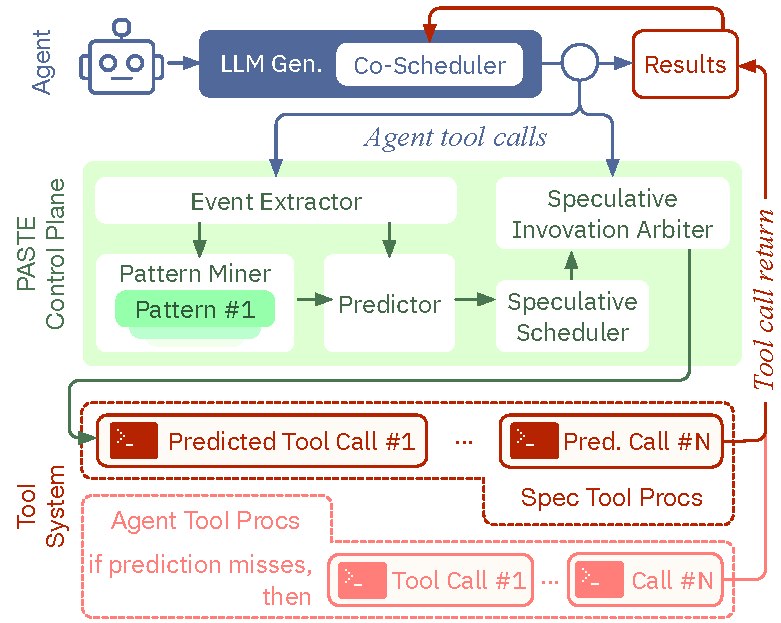
\includegraphics[width=\linewidth]{images/ATC/PASTE-v2.pdf}
    \caption{System architecture of \sys. \sys places a session-level control plane across the agent runtime, tool executor, and LLM serving engine.}
    \label{fig:system}
    \vspace{-0.12in}
\end{figure}

Figure~\ref{fig:system} shows the architecture of \sys.
Rather than treating the LLM engine and tool executor as independent services, \sys interposes a session-level control plane across the agent runtime, tool executor, and LLM serving engine.
Each agent request becomes an event stream with LLM turns, tool calls, tool outputs, timing signals, and session metadata.
The stream links the semantic LLM--tool loop to the physical serving timeline: \sys does not change which action the agent takes, but changes when predictable tool work runs and when completed sessions re-enter the LLM engine.

\noindent\textbf{Pattern Analyzer for concrete future invocations.}
The Pattern Analyzer converts recurring session structure into speculative invocation candidates.
It matches recent session history against recurring sub-workflows and, when the needed inputs are already present, instantiates the arguments required to execute the predicted invocation.

\noindent\textbf{Tool Speculation Scheduler for selective, interference-free overlap.}
The Tool Speculation Scheduler controls the speculative lifecycle.
It admits candidates according to confidence, expected benefit, and resource availability.
Authoritative tool invocations remain correctness-critical and keep priority.
Speculative work is bounded, deprioritized, or preempted under resource contention.
Speculative results stay outside authoritative session state until the LLM emits a matching invocation.
Tools with side effects require policy approval or a non-mutating variant.

\noindent\textbf{LLM--Tool Co-Scheduler for LLM-side pacing.}
The LLM--Tool co-scheduler paces sessions returned from the tool side to the LLM side.
It schedules LLM calls based on both authoritative and speculative tool execution signals, so that the active LLM load is optimal.
% It consumes authoritative and speculative tool-side signals, then admits completed or promoted sessions back to the LLM engine when doing so keeps active LLM load near the task-optimal region.

Together, these components create two complementary effects.
Intra-session overlap hides future tool latency, while cross-session pacing keeps the LLM engine in a latency-efficient region.

\subsection{Core Design Mechanisms}
\label{sec:overview-mechanisms}

This section summarizes the three core mechanisms; System Design details appear in \S\ref{sec:design}.

\subsubsection{Pattern-Aware Intra-Session Speculation}
\label{sec:overview-pattern-spec}

This mechanism creates overlap from predictable agent structure.
\sys learns recurring sub-workflows and implicit argument dependencies from prior sessions, then watches each live session for similar contexts.
When the required inputs already appear in the current session history, the Pattern Analyzer emits a concrete predicted invocation that can run while the LLM is still generating.
The design separates stable structure from volatile content: a search--visit pattern predicts that a web-fetch call is likely, but the concrete URL is copied from the current search output rather than guessed.

\subsubsection{Non-Interference Speculation Lifecycle}
\label{sec:overview-spec-lifecycle}

The speculation lifecycle separates best-effort predicted work from the authoritative path produced by the LLM.
A speculative invocation may start early, but it is not an agent-visible action until the LLM emits a matching authoritative invocation.
If the prediction matches, \sys reuses a completed result or promotes an in-flight job; if it misses, the work is discarded without changing session state.

\sys enforces two forms of non-interference.
\textbf{Resource side.} \sys prevents speculative jobs from delaying authoritative tool execution across concurrent sessions: authoritative jobs keep priority, and speculative jobs use only bounded or opportunistic capacity.
\textbf{Correctness side.} \sys prevents speculation from changing the agent outcome before confirmation: speculative results stay outside authoritative session state, and tools with side effects require an explicit safe-speculation policy or a non-mutating transformed execution.

\subsubsection{Joint LLM--Tool Co-Scheduling}
\label{sec:overview-coscheduling}

Joint LLM--tool co-scheduling converts local tool overlap into end-to-end latency reduction.
Speculation changes not only tool completion time, but also when sessions return to the LLM engine.
Without pacing, many sessions can become ready for generation at once, turning saved tool time into extra LLM queueing or decoding.
The LLM--Tool Co-Scheduler therefore observes tool completions, promoted jobs, active LLM requests, decode batch pressure, context length, and KV pressure.
It admits returning LLM turns so that exposed-tool-time reductions are preserved while the LLM engine stays near its task-optimal operating region.
